\section{Approach}\label{s:approach}

We argue that creating a categorical split between LC and BE in the scheduler
solves these problems (\autoref{ss:new-interface}). And in fact, the
infrastructure to enforce categorical separation already exists in Linux, and it
works remarkably well (\autoref{ss:sched-rt})

\subsection{A better interface: categorical separation}\label{ss:new-interface}

A categorical differentiation in the scheduler allows for fewer synchronization
points without compromising the enforcement of global isolation. In order to
enforce a categorical priority, the scheduler only needs to sychronize at two
points: on \textit{entry}, when a new high-priority thread wakes up on a core
already running something high-priority, and \textit{exit}, when starting to run
a low priority thread. If on entry the scheduler looks for cores running low
priority work to go interrupt, and on exit the scheduler looks for high priority
work to steal, it has ensured the global property that \textit{no core is ever
running a BE process while an LC one is runnable and waiting}.

This also has the added benefit that it can side-step the scheduling quantum
problem: the places where the scheduler needs to change which category it is
running are defined by wakeups and thread exit/blocking, which are points where
the scheduler is already running immediately, and can interpose and schedule.
Thus the fidelity of the isolation between separate categories is independent
from the size of the scheduling tick.


\subsection{Scheduling Classes isolate well}\label{ss:sched-rt}

There already exists a way to configure tasks to be categorically distinct in a
way that Linux enforces globally: processes that run in real time have strict
priority over other processes.

Linux does this by using \textit{scheduling classes}. Each scheduling class
exists completely separately: classes maintain their own runqueues and
per-entity state; implement their own scheduling algorithms to choose from the
entities on their runqueue; and balance the load across runqueues on different
cores.

Linux isolates strictly between different scheduling classes: it only schedules
a lower scheduling class if the higher scheduling classes found nothing to run,
and each scheduling class tries to steal work from other cores before returning
that it has nothing to run --- these two checks represent the entry and exit
synchronization points. It is thereby true that if something in the Normal
scheduling class is running, it means there are no Fifo tasks waiting to run
anywhere on the machine.

This points to a possible solution: run LC in the Fifo scheduling class and BE
in Normal.\footnote{The Deadline scheduling class is not a good fit, since it
requires accurate knowledge of a processes runtime (processing time per request)
and period (when requests come in)} Fifo runs a priority scheduler: it has 99
priorities, each takes strict precedent over the one lower; within priorities
the scheduler enforces a global first-in-first-out (hence the Fifo class name),
based on when processes become runnable.

\begin{figure}[t]
    \centering
    \begin{subfigure}[t]{0.48\columnwidth}
        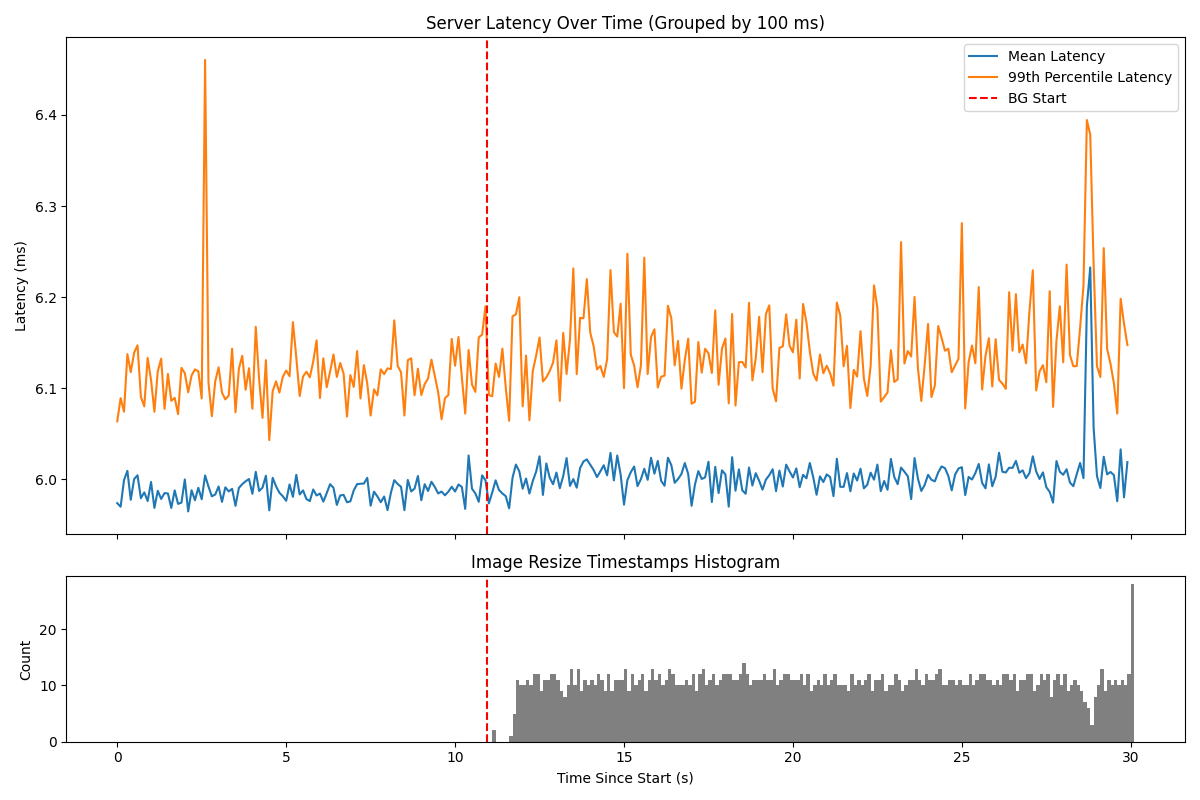
\includegraphics[width=\columnwidth]{graphs/unedited-rt-low-two.png}
        \caption{Low load}\label{fig:unedited-rt-low-two}
    \end{subfigure}
    \hspace{\fill}
    \begin{subfigure}[t]{0.48\columnwidth}
        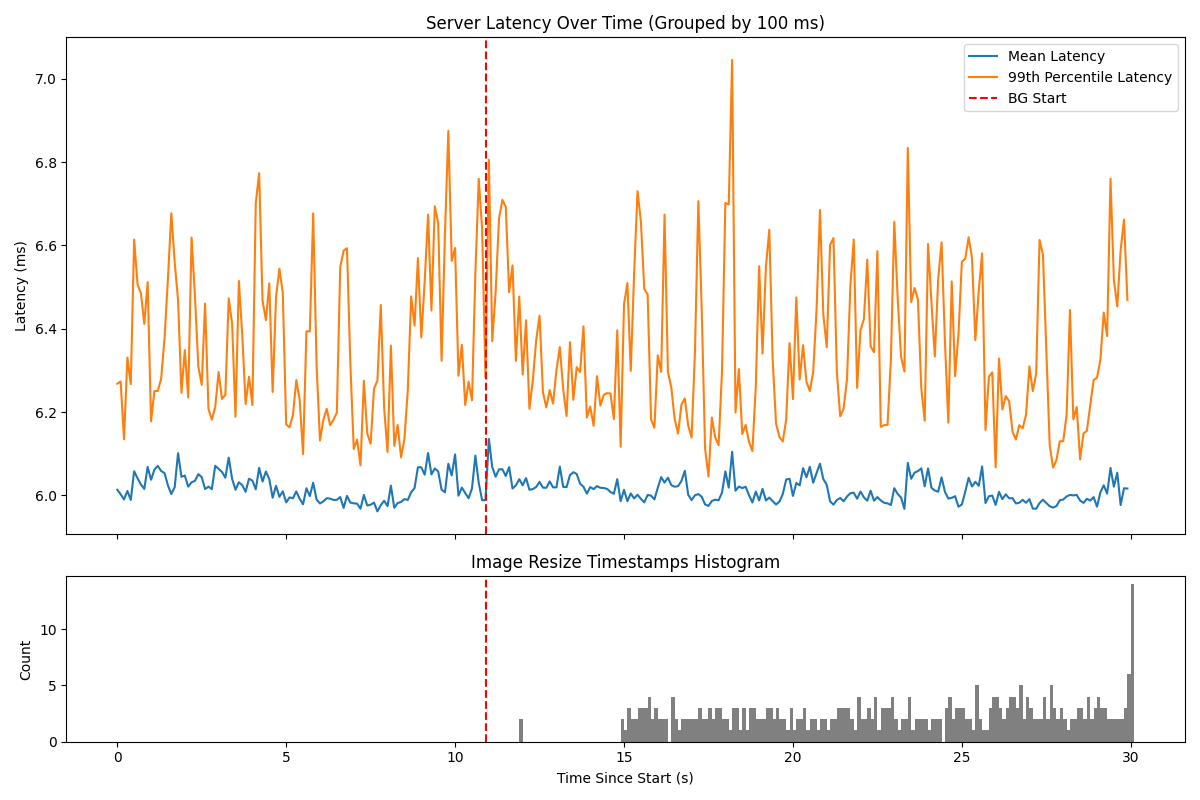
\includegraphics[width=\columnwidth]{graphs/unedited-rt-high-two.png}
        \caption{High load}\label{fig:unedited-rt-high-two}
    \end{subfigure}
    \vspace{4pt}
    \caption{Results of the same experiment, with LC running as a real time process}\label{fig:unedited-rt}
\end{figure}

We run the same experiment as in \autoref{s:intro}, but put the LC task in the
Fifo scheduling class, and leave BE tasks with the default process weight.
\autoref{fig:unedited-rt} shows the resulting measured latencies in the same low
and high load setting as previously. As expected, we see that Linux is able to
isolate the two very well. 

However, this is an untenable final solution because of Fifo's run-to-completion
scheduling, which is known to have a failure mode of head-of-line (HoL) blocking
under varied request processing times, where long-running requests monopolize
the CPU while short requests wait in the queue. The Fifo scheduler also enforces
not only cross-core isolation between different priorities, but also a global
ordering within the same priority.

The takeaway is that Linux's current mechanism of scheduling classes can isolate
workloads effectively, but existing scheduling classes use scheduling
algorithms that are not a good fit for modern workloads.

\subsection{Be: A new scheduling class}


\hmng{I'm trying something by moving this in here, but from here on out the
structure gets kinda weird/is not the standard paper structure. It seems to me
that the pieces we need to hit before eval are: our solution is a new, lower,
scheduling class; \schedidle{} already exists but doesn't work; we patch it up
so that it does}

In order to have the benefits of categorical separation while maintaining the
expected Processor Sharing scheduler for the LC services, we propose creating a
new scheduling class, Be, that exists below the Normal scheduling class.



